\documentclass{article}

\usepackage[most]{tcolorbox}
\usepackage{physics}
\usepackage{graphicx}
\usepackage{float}
\usepackage{amsmath}
\usepackage{amssymb}


\usepackage[utf8]{inputenc}
\usepackage[a4paper, margin=1in]{geometry} % Controla los márgenes
\usepackage{titling}

\title{Clase 17 }
\author{Manuel Garcia.}
\date{\today}

\renewcommand{\maketitlehooka}{%
  \centering
  \vspace*{0.05cm} % Espacio vertical antes del título
}

\renewcommand{\maketitlehookd}{%
  \vspace*{2cm} % Espacio vertical después de la fecha
}

\newcommand{\caja}[3]{%
  \begin{tcolorbox}[colback=#1!5!white,colframe=#1!25!black,title=#2]
    #3
  \end{tcolorbox}%
}

\begin{document}
\maketitle

\section{Integración compleja }
\subsection{Trayecto o contorno }
Llamaremos curva a una función $ y = f(x)  $, continua. esta curva puede ser expresada en forma paramétrica, de tal manera, que $ x  $ e $ y  $ son funciones de un nuevo parámetro $ t  $. 

\textbf{Por ejemplo } consideremos una semicricunferencia unitaria descrita por $ y = \sqrt{1 - x ^2}  $, con $ -1 \leq x \leq 1  $. Su parametrizacion es: 
\begin{gather*}
  x  = x(t)= \cos{t }, \qquad y = y(t) = \sin{t }, \qquad t \in [0,\pi ] 
\end{gather*}
De esta manera, se debe poner atención en que si se recorre $ t  $ de menor a mayor, $ x  $ se recorreria de mayor a menor. Definiremos esta direccion de barrido , como direccion positiva.
\begin{figure}[H]
  \begin{center}
    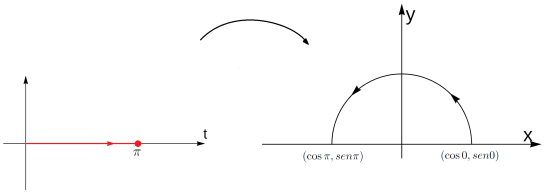
\includegraphics[width=0.6\textwidth]{contorno_integracion.png}
  \end{center}
\end{figure}
Claramente, si se barriera $ r  $ de maor a menor, $ x  $ se barrería de menor a mayor (barrido en dirección negariva, sentido de las manecillas de reloj).

Ahora tendremos una curva cerrada, si el valor en sus extremos coincide. $ \gamma(t), a \leq t \leq b  $, será cerrada si $ \gamma(a) = \alpha(b)  $.

"Una curva puede tener multiples parametrizaciones", Ej: Parametricemos $ [0,1] $: 
\begin{gather*}
  \gamma_1(t) = t, 0 \leq t \leq 1 \qquad \qquad \gamma_2 (t) = t ^2, 0\leq t \leq 1 
\end{gather*}

Entonces, como $ z(t) = x(t) + i y (t)  \rightarrow  \gamma(t) = x(T) + i y (t) $

Algunas parametrizaciones útiles: 
\begin{itemize}
  \item Parametrización general de una circunferencia: $ (R>0 ) $
    \begin{align*}
      \gamma(t) &= z_0 + R e  ^ {i t } \\
           &= z_0 + R(\cos{t } + i \sin{t })\\
           &= x_0+iy_0 + R \cos{t } + i R \sin{t }\\
      x(t) &= x_0 + R \cos{t },\quad  y(t) = y_0 + R \sin{t }
    \end{align*}
    \textbf{Ejemplo: }Parametrizar, la circunferencia con $ R=3  $ y centro en $ z_0 = e ^ {3i } $
    \begin{gather*}
      x(t) = \cos{3 } + 3 \cos{t }, \quad y(t) = \sin{3 } + 3 \sin{t } , \quad 0 \leq t \leq 2\pi
    \end{gather*}
  \item Parametrización d eun segmento de reca: 

    Sean los extremos del segmento en $ z_1  $ y $ z_2  $. Una parametrización posibles, es : 
    \begin{gather*}
      \gamma(t) = (1-t)z_1 + t z_2 ,\quad 0\leq t \leq 1  
    \end{gather*}
  \item Parametrizacion de fitura de lsajous
    \begin{gather*}
      x(t) = \sin{2t } \quad \text{ y } \quad y(t) = \sin{3t } \qquad 0\leq t \leq 2 \pi 
    \end{gather*}
    \begin{figure}[H]
      \begin{center}
        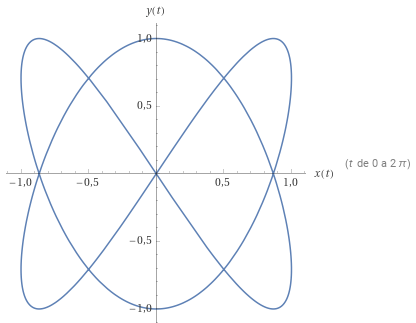
\includegraphics[width=0.35\textwidth]{lisajous.png}
      \end{center}
    \end{figure}
\end{itemize}

De manera sistematica se puede cambiar la orientación de barrido, por ejemplo de positiva a negativa, si $ t\in [a,b] $ entonces sustituyo el parametro por $ a + b - t \in [b,a] $

\textbf{Ejemplo } Sea el trayecto $ \gamma (t) = 2-i + 3 e ^ {i t }, \quad t \in [0,2\pi ] $.
\begin{gather*}
  \gamma_1 (t) = 2- i + 3 e ^ {i(2\pi - t)}, \quad a= 0 , \quad b= 2\pi
\end{gather*}

\hfill 

\hfill

\hfill

Resaltemos lo que implica una funcion compleja de una variable real. En este caso vamos a tener lo siguiente: 
\begin{gather*}
  f'(t) = \frac{d f(t)  }{d t } = \underset{h \rightarrow 0 }{lim } \frac{f(t+h ) - f(t) }{h }, \qquad f'(t) = Re\{f' \} + i Im \{f' \}
\end{gather*}

\textbf{Propiedades: }
\begin{itemize}
  \item $ (\alpha f + \beta g )' = \alpha f' + \beta g'  $ con $ \alpha,\beta \in \mathbb{C}, \quad f(t),g(t), \quad t \in (a,b)  $
  \item $ (f \cdot g)' = fg' + f'g  $
  \item $\left(\frac{f }{g }\right)' = \frac{g f' - f g' }{g^2 }, g(t) \neq 0 $ 
  \item $(f \circ h)' = f'(h(t)) \cdot h'(t)$
    \textbf{EJ: } $ \text{si: }f(t) = \sin{3zt }\quad \rightarrow \quad f'(t) = 3z \cos{3zt } $
    \begin{gather*}
      f'(t) = \underset{h  \rightarrow 0 }{lim}\frac{\sin{3z(t + h )} - \sin{3zt }}{h } 
    \end{gather*}
\end{itemize}


\end{document}
